\documentclass{beamer}
\usepackage[utf8]{inputenc}

\usetheme{Madrid}
\usecolortheme{default}
\usepackage{amsmath,amssymb,amsfonts,amsthm}
\usepackage{txfonts}
\usepackage{tkz-euclide}
\usepackage{listings}
\usepackage{adjustbox}
\usepackage{array}
\usepackage{tabularx}
\usepackage{gvv}
\usepackage{lmodern}
\usepackage{circuitikz}
\usepackage{tikz}
\usepackage{graphicx}

\setbeamertemplate{page number in head/foot}[totalframenumber]

\usepackage{tcolorbox}
\tcbuselibrary{minted,breakable,xparse,skins}



\definecolor{bg}{gray}{0.95}
\DeclareTCBListing{mintedbox}{O{}m!O{}}{%
	breakable=true,
	listing engine=minted,
	listing only,
	minted language=#2,
	minted style=default,
	minted options={%
		linenos,
		gobble=0,
		breaklines=true,
		breakafter=,,
		fontsize=\small,
		numbersep=8pt,
		#1},
	boxsep=0pt,
	left skip=0pt,
	right skip=0pt,
	left=25pt,
	right=0pt,
	top=3pt,
	bottom=3pt,
	arc=5pt,
	leftrule=0pt,
	rightrule=0pt,
	bottomrule=2pt,
	toprule=2pt,
	colback=bg,
	colframe=orange!70,
	enhanced,
	overlay={%
		\begin{tcbclipinterior}
			\fill[orange!20!white] (frame.south west) rectangle ([xshift=20pt]frame.north west);
	\end{tcbclipinterior}},
	#3,
}
\lstset{
	language=C,
	basicstyle=\ttfamily\small,
	keywordstyle=\color{blue},
	stringstyle=\color{orange},
	commentstyle=\color{green!60!black},
	numbers=left,
	numberstyle=\tiny\color{gray},
	breaklines=true,
	showstringspaces=false,
}
%------------------------------------------------------------
%This block of code defines the information to appear in the
%Title page
\title %optional
{2.10.65}
\date{}
%\subtitle{A short story}

\author % (optional)
{M Chanakya Srinivas- EE25BTECH11036}




\begin{document}


\frame{\titlepage}






\begin{frame}{Problem Statement}
Let \(OACB\) be a parallelogram with \(O\) at the origin and \(OC\) a diagonal.\\
Let \(D\) be the midpoint of \(OA\).\\
Using vector methods, prove that \(BD\) and \(CO\) intersect in the same ratio. Determine this ratio.
\end{frame}

\begin{frame}{Step 1: Define position vectors}
\begin{align}
\vec{O} &= \myvec{0\\0}, \\
\vec{A} &= \vec{a}, \\
\vec{C} &= \vec{c}, \\
\vec{B} &= \vec{A} + \vec{C}, \\
\vec{D} &= \frac{\vec{O} + \vec{A}}{2} = \frac{1}{2}\vec{A}.
\end{align}
\end{frame}

\begin{frame}{Step 2: Vector equations of lines}
\textbf{Line \(BD\):}
\begin{align}
\vec{R_1} &= \vec{B} + \lambda (\vec{D} - \vec{B}) \\
&= \vec{B} - \lambda \left(\frac{1}{2}\vec{A} + \vec{C}\right)
\end{align}

\textbf{Line \(CO\):}
\begin{align}
\vec{R_2} &= \vec{C} + \mu (\vec{O} - \vec{C}) = (1-\mu)\vec{C}
\end{align}
\end{frame}

\begin{frame}{Step 3: Intersection condition}
\[
\vec{R_1} = \vec{R_2} \quad \Rightarrow \quad 
\vec{B} - \lambda \left(\frac{1}{2}\vec{A} + \vec{C}\right) = (1-\mu)\vec{C}
\]

Substitute \(\vec{B} = \vec{A} + \vec{C}\):
\[
\vec{A} + \vec{C} - \lambda \left(\frac{1}{2}\vec{A} + \vec{C}\right) = (1-\mu)\vec{C}
\]
\end{frame}

\begin{frame}{Step 4: Equate coefficients of vectors}
\begin{align}
\text{Coefficient of } \vec{A}: & \quad 1 - \frac{\lambda}{2} = 0 \quad \Rightarrow \quad \lambda = 2 \\
\text{Coefficient of } \vec{C}: & \quad 1 - \lambda = 1 - \mu \quad \Rightarrow \quad \mu = 2
\end{align}
\end{frame}

\begin{frame}{Step 5: Interpret the ratio}
\begin{itemize}
\item On \(BD\), \(\lambda = 2\) \(\Rightarrow\) intersection divides \(BD\) in ratio \(2:1\).  
\item On \(CO\), \(\mu = 2\) \(\Rightarrow\) intersection divides \(CO\) in ratio \(2:1\).  
\end{itemize}

\begin{align}
\boxed{\text{The lines $BD$ and $CO$ intersect in the ratio } 2:1.}
\end{align}
\end{frame}






\begin{frame}[fragile]{C code}
\begin{lstlisting}
// parallelogram.c
#include <stdio.h>
typedef struct {
    double x;
    double y;
} Point;
static Point result;
Point intersection() {
    Point O = {0.0, 0.0};
    Point A = {1.0, 0.0};
    Point B = {0.0, 1.0};
    Point D = {(O.x + A.x)/2.0, (O.y + A.y)/2.0};
    double lam = 2.0/3.0;
    result.x = B.x + lam * (D.x - B.x);
    result.y = B.y + lam * (D.y - B.y);
  return result;
}
\end{lstlisting}
\end{frame}
\begin{frame}[fragile]{Python code through shared output}
\begin{lstlisting}
import ctypes
import matplotlib.pyplot as plt
import numpy as np
# Load the shared library
lib = ctypes.CDLL("./libparallelogram.so")
# Define return type for the intersection function
class Point(ctypes.Structure):
    _fields_ = [("x", ctypes.c_double), ("y", ctypes.c_double)]
lib.intersection.restype = Point
# Get intersection P
P = lib.intersection()
print("Intersection P =", (P.x, P.y))
# Define points
O = np.array([0, 0])
A = np.array([1, 0])
B = np.array([0, 1])
C = A + B
D = (O + A)/2
P_vec = np.array([P.x, P.y])
\end{lstlisting}
\end{frame}
\begin{frame}[fragile]{Python code through shared output}
\begin{lstlisting}
# --- Plot ---
fig, ax = plt.subplots()
# Parallelogram
ax.plot([O[0], A[0], C[0], B[0], O[0]],
        [O[1], A[1], C[1], B[1], O[1]], 'k-')
# Diagonal OC
ax.plot([O[0], C[0]], [O[1], C[1]], 'r--', label="OC")
# Line BD
ax.plot([B[0], D[0]], [B[1], D[1]], 'g--', label="BD")
# Points
for Pnt, name in zip([O,A,B,C,D,P_vec], ['O','A','B','C','D','P']):
    ax.scatter(Pnt[0], Pnt[1], s=50)
    ax.text(Pnt[0]+0.05, Pnt[1]+0.05, name)
ax.set_aspect('equal')
ax.legend()
plt.title("Intersection of BD and CO in ratio 2:1")
plt.show()
\end{lstlisting}
\end{frame}
\begin{frame}[fragile]{only Python code}
\begin{lstlisting}
import sys
sys.path.insert(0, '/sdcard/github/matgeo/codes/CoordGeo')  # path to CoordGeo
import numpy as np
import matplotlib.pyplot as plt
import subprocess
import shlex
import os  # << add this
# Local imports
from line.funcs import line_gen
# Define points as column vectors
O = np.array([[0], [0]])
A = np.array([[1], [0]])
B = np.array([[0], [1]])
C = A + B
D = (O + A) / 2
# Compute intersection P on BD such that P = B + (2/3)(D - B)
lam = 2/3
P = B + lam * (D - B)
# Generate required lines
x_OC = line_gen(O, C)
x_BD = line_gen(B, D)
\end{lstlisting}
\end{frame}
\begin{frame}[fragile]{only Python code}
\begin{lstlisting}
# Parallelogram edges
x_OA = line_gen(O, A)
x_AB = line_gen(A, C)
x_CB = line_gen(C, B)
x_BO = line_gen(B, O)
plt.plot(x_OC[0,:], x_OC[1,:], 'r--', label='$OC$')
plt.plot(x_BD[0,:], x_BD[1,:], 'g--', label='$BD$')
for line in [x_OA, x_AB, x_CB, x_BO]:
    plt.plot(line[0,:], line[1,:], 'k-')
coords = np.block([[O, A, B, C, D, P]])
labels = ['O', 'A', 'B', 'C', 'D', 'P']
plt.scatter(coords[0,:], coords[1,:])
for i, txt in enumerate(labels):
    plt.annotate(f'{txt}\n({coords[0,i]:.2f}, {coords[1,i]:.2f})',
                 (coords[0,i], coords[1,i]),
                 textcoords="offset points",
                 xytext=(10,-10),
                 ha='center')
\end{lstlisting}
\end{frame}
\begin{frame}[fragile]{only Python code}
\begin{lstlisting}
# Styling
ax = plt.gca()
ax.spines['left'].set_visible(False)
ax.spines['right'].set_visible(False)
ax.spines['top'].set_visible(False)
ax.spines['bottom'].set_visible(False)
plt.axis('equal')
plt.grid()
plt.legend(loc='best')
plt.title("Intersection of BD and OC (Pure Python)")
# Create directory if needed and save figure
save_path = 'chapters/10/7/2/2/figs/fig.pdf'
os.makedirs(os.path.dirname(save_path), exist_ok=True)
plt.savefig(save_path)
try:
    subprocess.run(shlex.split(f"termux-open {save_path}"))
except:
    plt.show()
\end{lstlisting}
\end{frame}
\begin{frame}[fragile]{PLOTS}
\begin{figure}
    \centering
    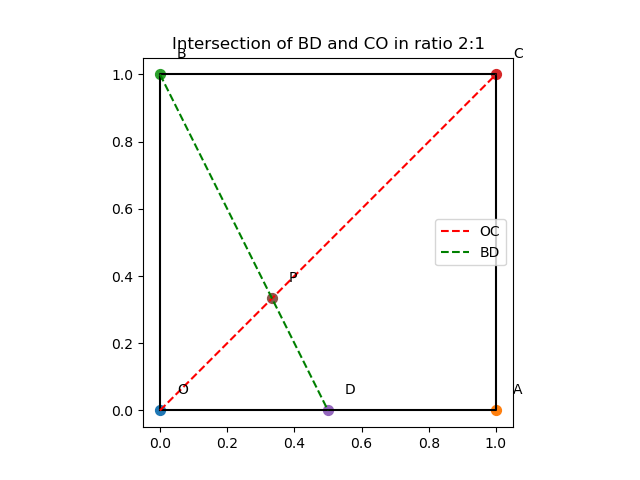
\includegraphics[width=0.9\columnwidth]{figs/fig51.png}
    \caption{}
    \label{fig:placeholder}
\end{figure}
\end{frame}
\begin{frame}[fragile]{PLOTS}
\begin{figure}
    \centering
    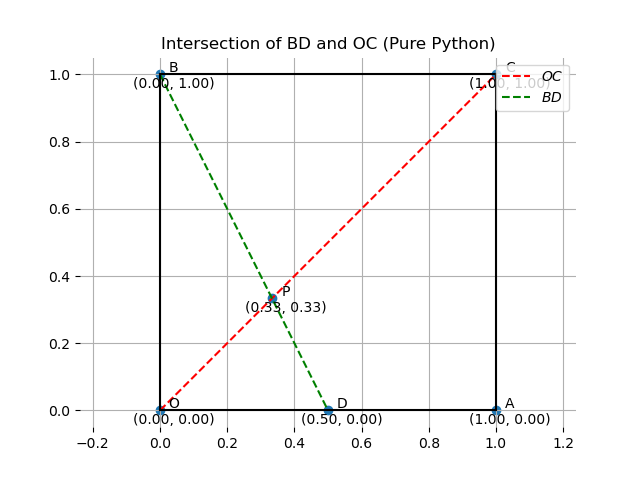
\includegraphics[width=0.9\columnwidth]{figs/fig52.png}
    \caption{}
    \label{fig:placeholder}
\end{figure}
\end{frame}
\end{document}